\chapter{7 TeV and 8 TeV Differential Cross Section: Systematic Uncertainties and Results}
\label{c:Differential_Cross_Section:systematics_and_results}

\section{Systematic uncertainties}
\label{s:systematic_uncertainties}
The systematic uncertainties in this analysis are evaluated independently, under the assumption that
systematic uncertainty sources are uncorrelated, by changing the inputs by the associated uncertainties
($-1\sigma$ and $+1\sigma$) and measuring the deviation in the final result from the nominal measurement. The
final result from systematic variations are generally found to be compatible with the nominal measurement within uncertainties. The
uncertainties from each source are therefore symmetrised by using the maximum absolute deviation of the up or
down systematic variation. The total systematic uncertainty is obtained by adding the systematic uncertainties
in quadrature, and this is summed with the fitting and unfolding uncertainties to obtain the total measurement
uncertainty. The normalisation of the final differential cross section will cancel systematic uncertainties
that are correlated between bins of the primary variables.

In the case of experimental uncertainties, the uncertainty is calculated by changing the templates in the
fitting process and/or their normalisations, and using the nominal \MADGRAPH response matrix in the unfolding
process. In the case of theoretical uncertainties, the central fitting templates and normalisation are used,
while the response matrix information is changed according to the systematic being investigated.

The systematic uncertainties are summarised in Tables~\ref{tab:MET_systematics_7TeV_combined} to
\ref{tab:MT_systematics_8TeV_combined}.

\subsection{Experimental Uncertainties}
\label{ss:experimental_uncertainties}

Jet energy scale uncertainty is evaluated as a function of jet \pt and jet $\eta$, and a 10\% jet energy
resolution uncertainty is applied. The jet energy scale (JES) directly changes the \pt of jets in
the event, and also propagates to the event \met (see
Section~\ref{ss:met_corrections}). Therefore the JES uncertainty becomes significant at higher
values of the primary variables, in particular of \met, \HT and \st.

Together with jet energy scale uncertainty, the \met energy uncertainties are the only systematics applied to
both simulation and data. These take account of uncertainty in the lepton energy, and propagates this to the
\met in the event. While the electron and muon energy uncertainties are not dominant sources of error in this
analysis, the effect of the uncertainty on tau energy has been calculated to be larger. Events with tau
leptons can pass the signal selection (a component of what are known as fake events, i.e. non semi-leptonic
\ttbar events which pass our signal selection) if they mimic the signature of an electron+jets or muon+jets
\ttbar event:

\begin{itemize}
 \item semi-leptonic tau, where $\tau \rightarrow e/\mu + \bar{\nu}_{e/\mu} + \nu_{\tau}$
 (Figure~\ref{subfig:semileptonic_tau_events}).
 \item di-leptonic $e\tau$ \& $\mu\tau$, where $\tau \rightarrow q\bar{q}^{'} + \nu_\tau$
 (Figure~\ref{subfig:dileptonic_tau_events_to_quarks}).
 \item di-leptonic $\tau\tau$, where $\tau \rightarrow q\bar{q}^{'} + \nu_\tau, \tau \rightarrow e/\mu
 + \bar{\nu}_{e/\mu}$ (Figure~\ref{subfig:semileptonic_tau_events_to_quarks_and_leptons}).
\end{itemize}

\begin{figure}%[!]
	\centering
	\subfloat[]{
		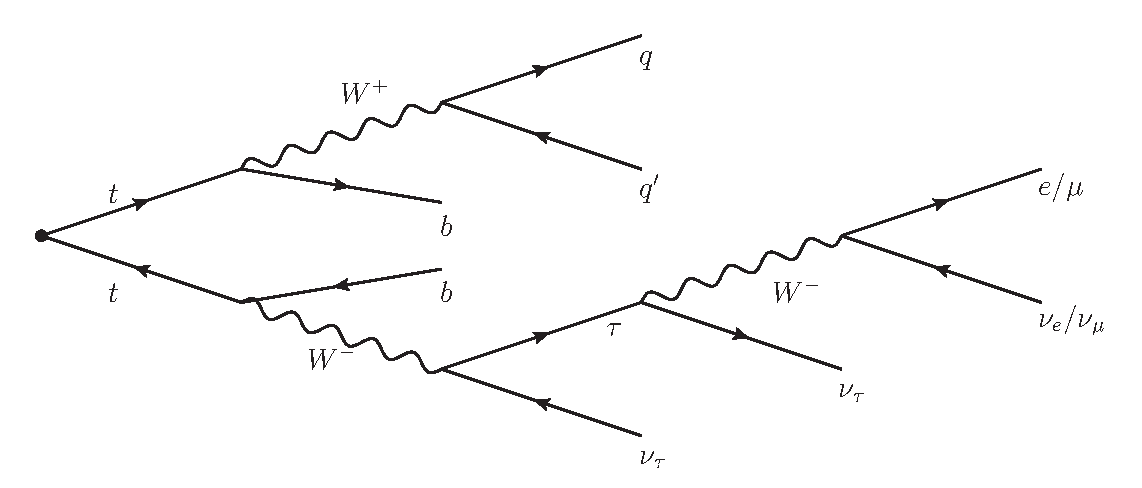
\includegraphics[width=0.45\textwidth]{Chapters/04_Analysis/04b_XSections/images/feynman_diagrams/semileptonic_tau_to_lepton}
%	\caption{}
		\label{subfig:semileptonic_tau_events}
		}
	\subfloat[]{
		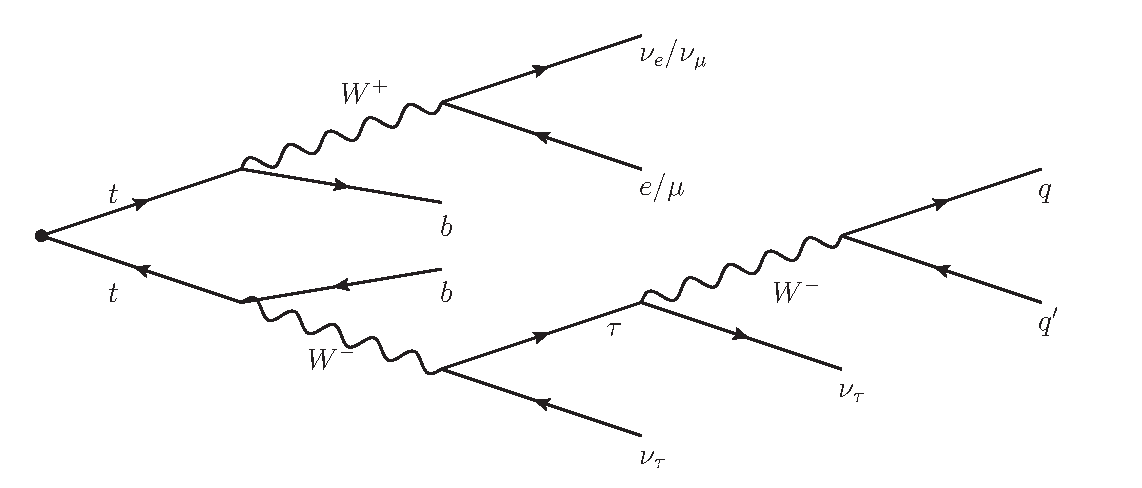
\includegraphics[width=0.45\textwidth]{Chapters/04_Analysis/04b_XSections/images/feynman_diagrams/dileptonic_tau_to_quarks}		
		\label{subfig:dileptonic_tau_events_to_quarks}
		}\\
	\subfloat[]{
		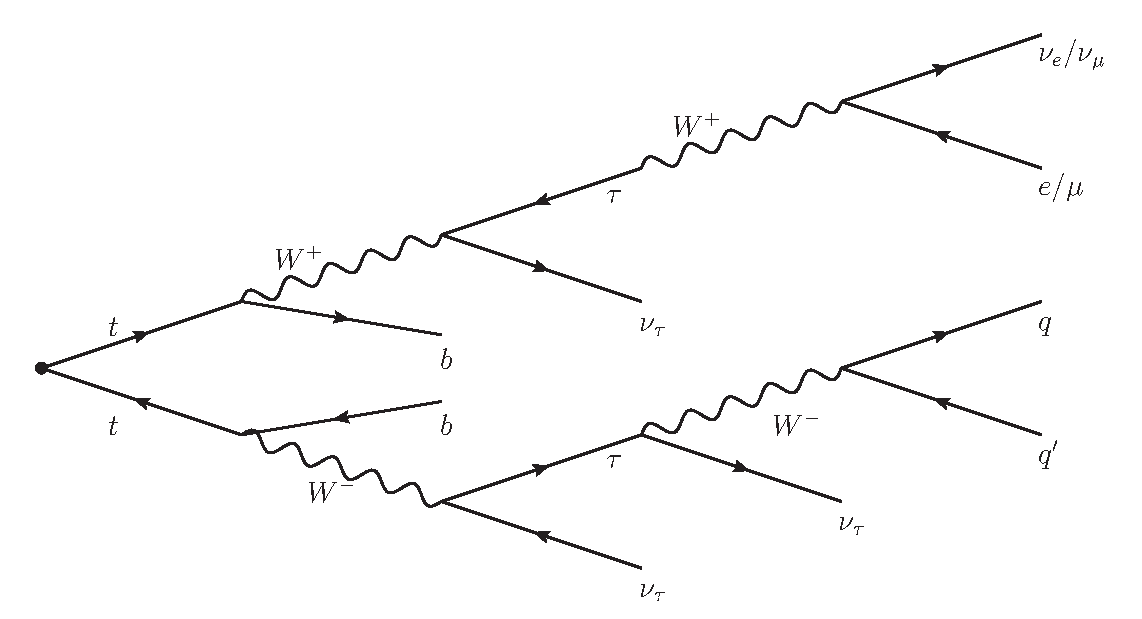
\includegraphics[width=0.45\textwidth]{Chapters/04_Analysis/04b_XSections/images/feynman_diagrams/dileptonic_tau_tau_to_quarks_and_leptons}
		\label{subfig:semileptonic_tau_events_to_quarks_and_leptons}
		}
	\caption[Diagrams of semi-leptonic and dileptonic $\tau$ events.]{Feynman diagrams of semi-leptonic $\tau$
	events (a), dileptonic events with one $\tau$ lepton (b) and dileptonic events with two $\tau$ leptons (c).}
	\label{fig:tau_diagrams}
\end{figure}

If, for example, the leptonically decaying \W boson from a semi-leptonic \ttbar decay decays to a tau lepton
and a tau neutrino, and the tau lepton then decays to another tau neutrino, an electron/muon and an electron
neutrino/muon neutrino via a virtual \W boson, such an event might fake our signal and pass the \ttbar signal
selection. Fake events are removed by subtracting the fake distribution obtained from simulation. However, for
the systematic measurements with the tau energy varied up and down, the same fake distribution shape is
subtracted as in the nominal measurement. A comparison of the fakes and the signal \met distributions shapes
from \ttbar simulation are shown on the left in Figure~\ref{fig:tau_shape_number_comparison}.
It can be seen that the relative contribution from fakes increases as \met increases. Approximately 14\% of
the reconstructed \ttbar events in simulation are fake events (13.5\% in electron channel and 13.9\% in muon
channel). The right hand plot in Figure~\ref{fig:tau_shape_number_comparison} compares the normalisations of
signal and fake events after selection. The effect of varying the electron and muon energies is not so
pronounced because there are not many electrons or muons in the fake collection (a dileptonic \ttbar event
with $ee$, $e\mu$ or $\mu\mu$ would have to be misreconstructed as a semi-leptonic event for this to happen).

\begin{figure}[hbtp]
    \centering
     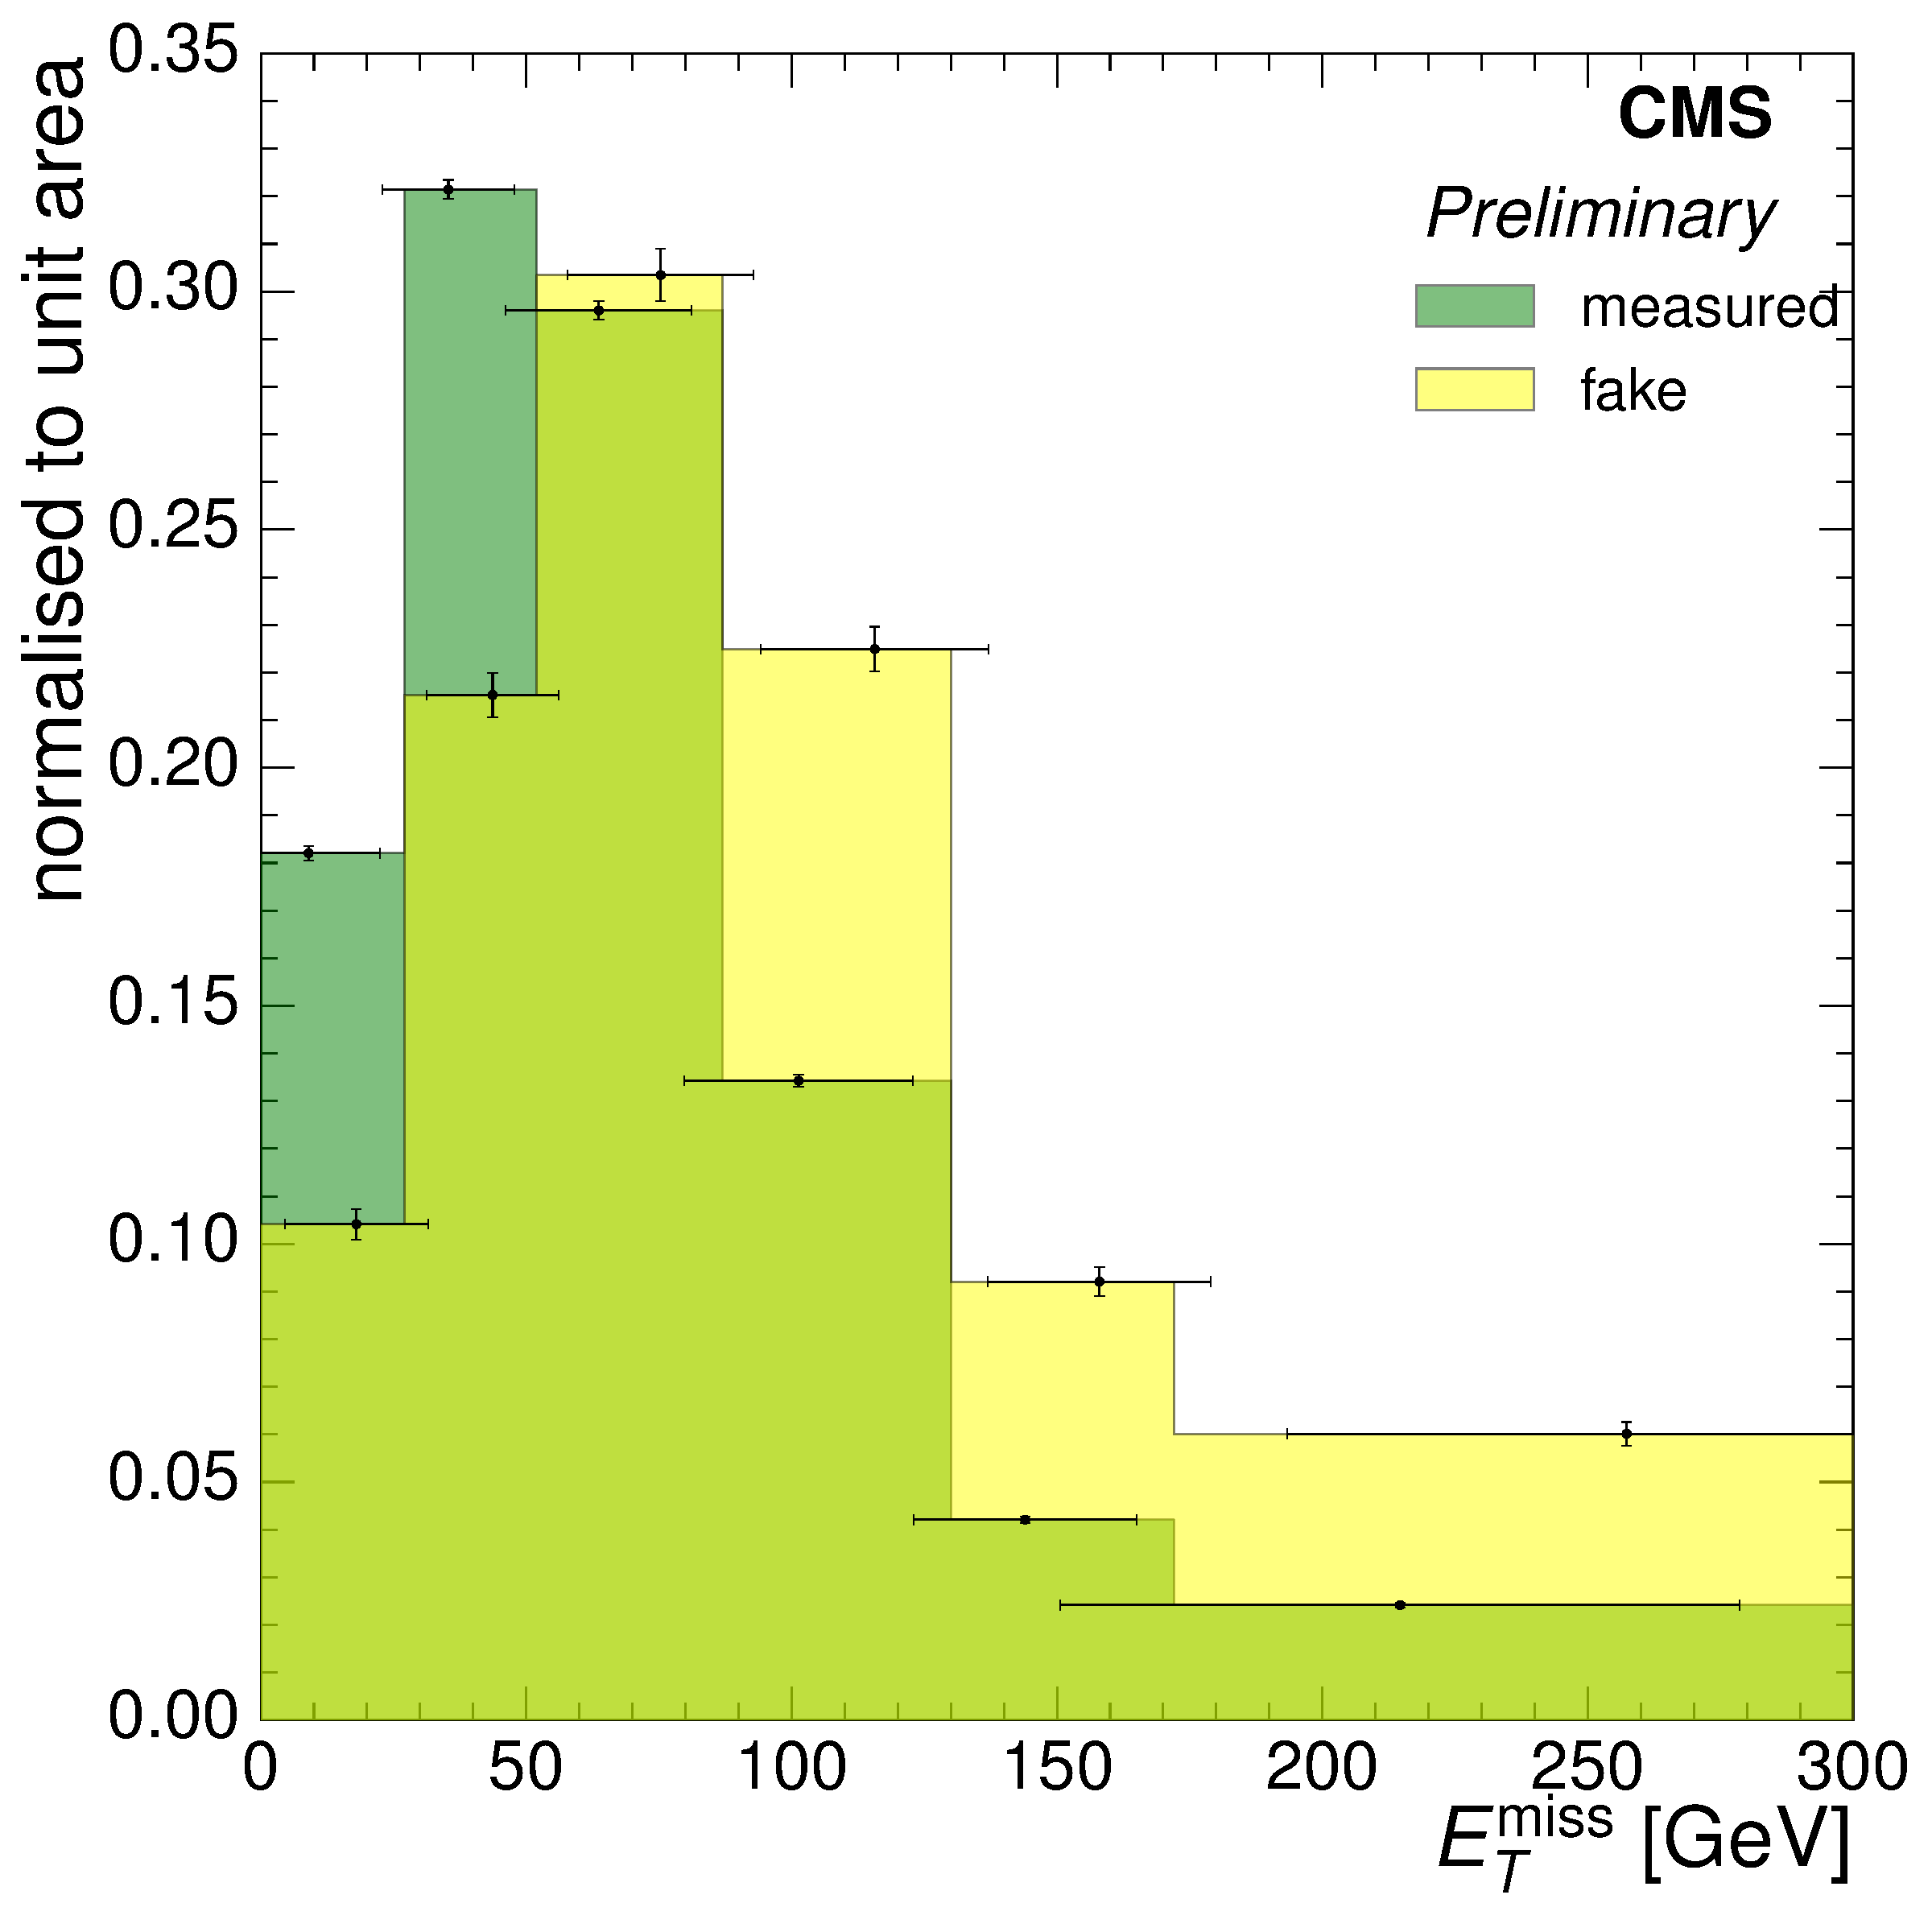
\includegraphics[width=0.48\textwidth]{Chapters/04_Analysis/04b_XSections/images/tau_cross_checks/comparison_measured_fake_TTJets_normalised_to_one_without_ratio.pdf}\hfill
     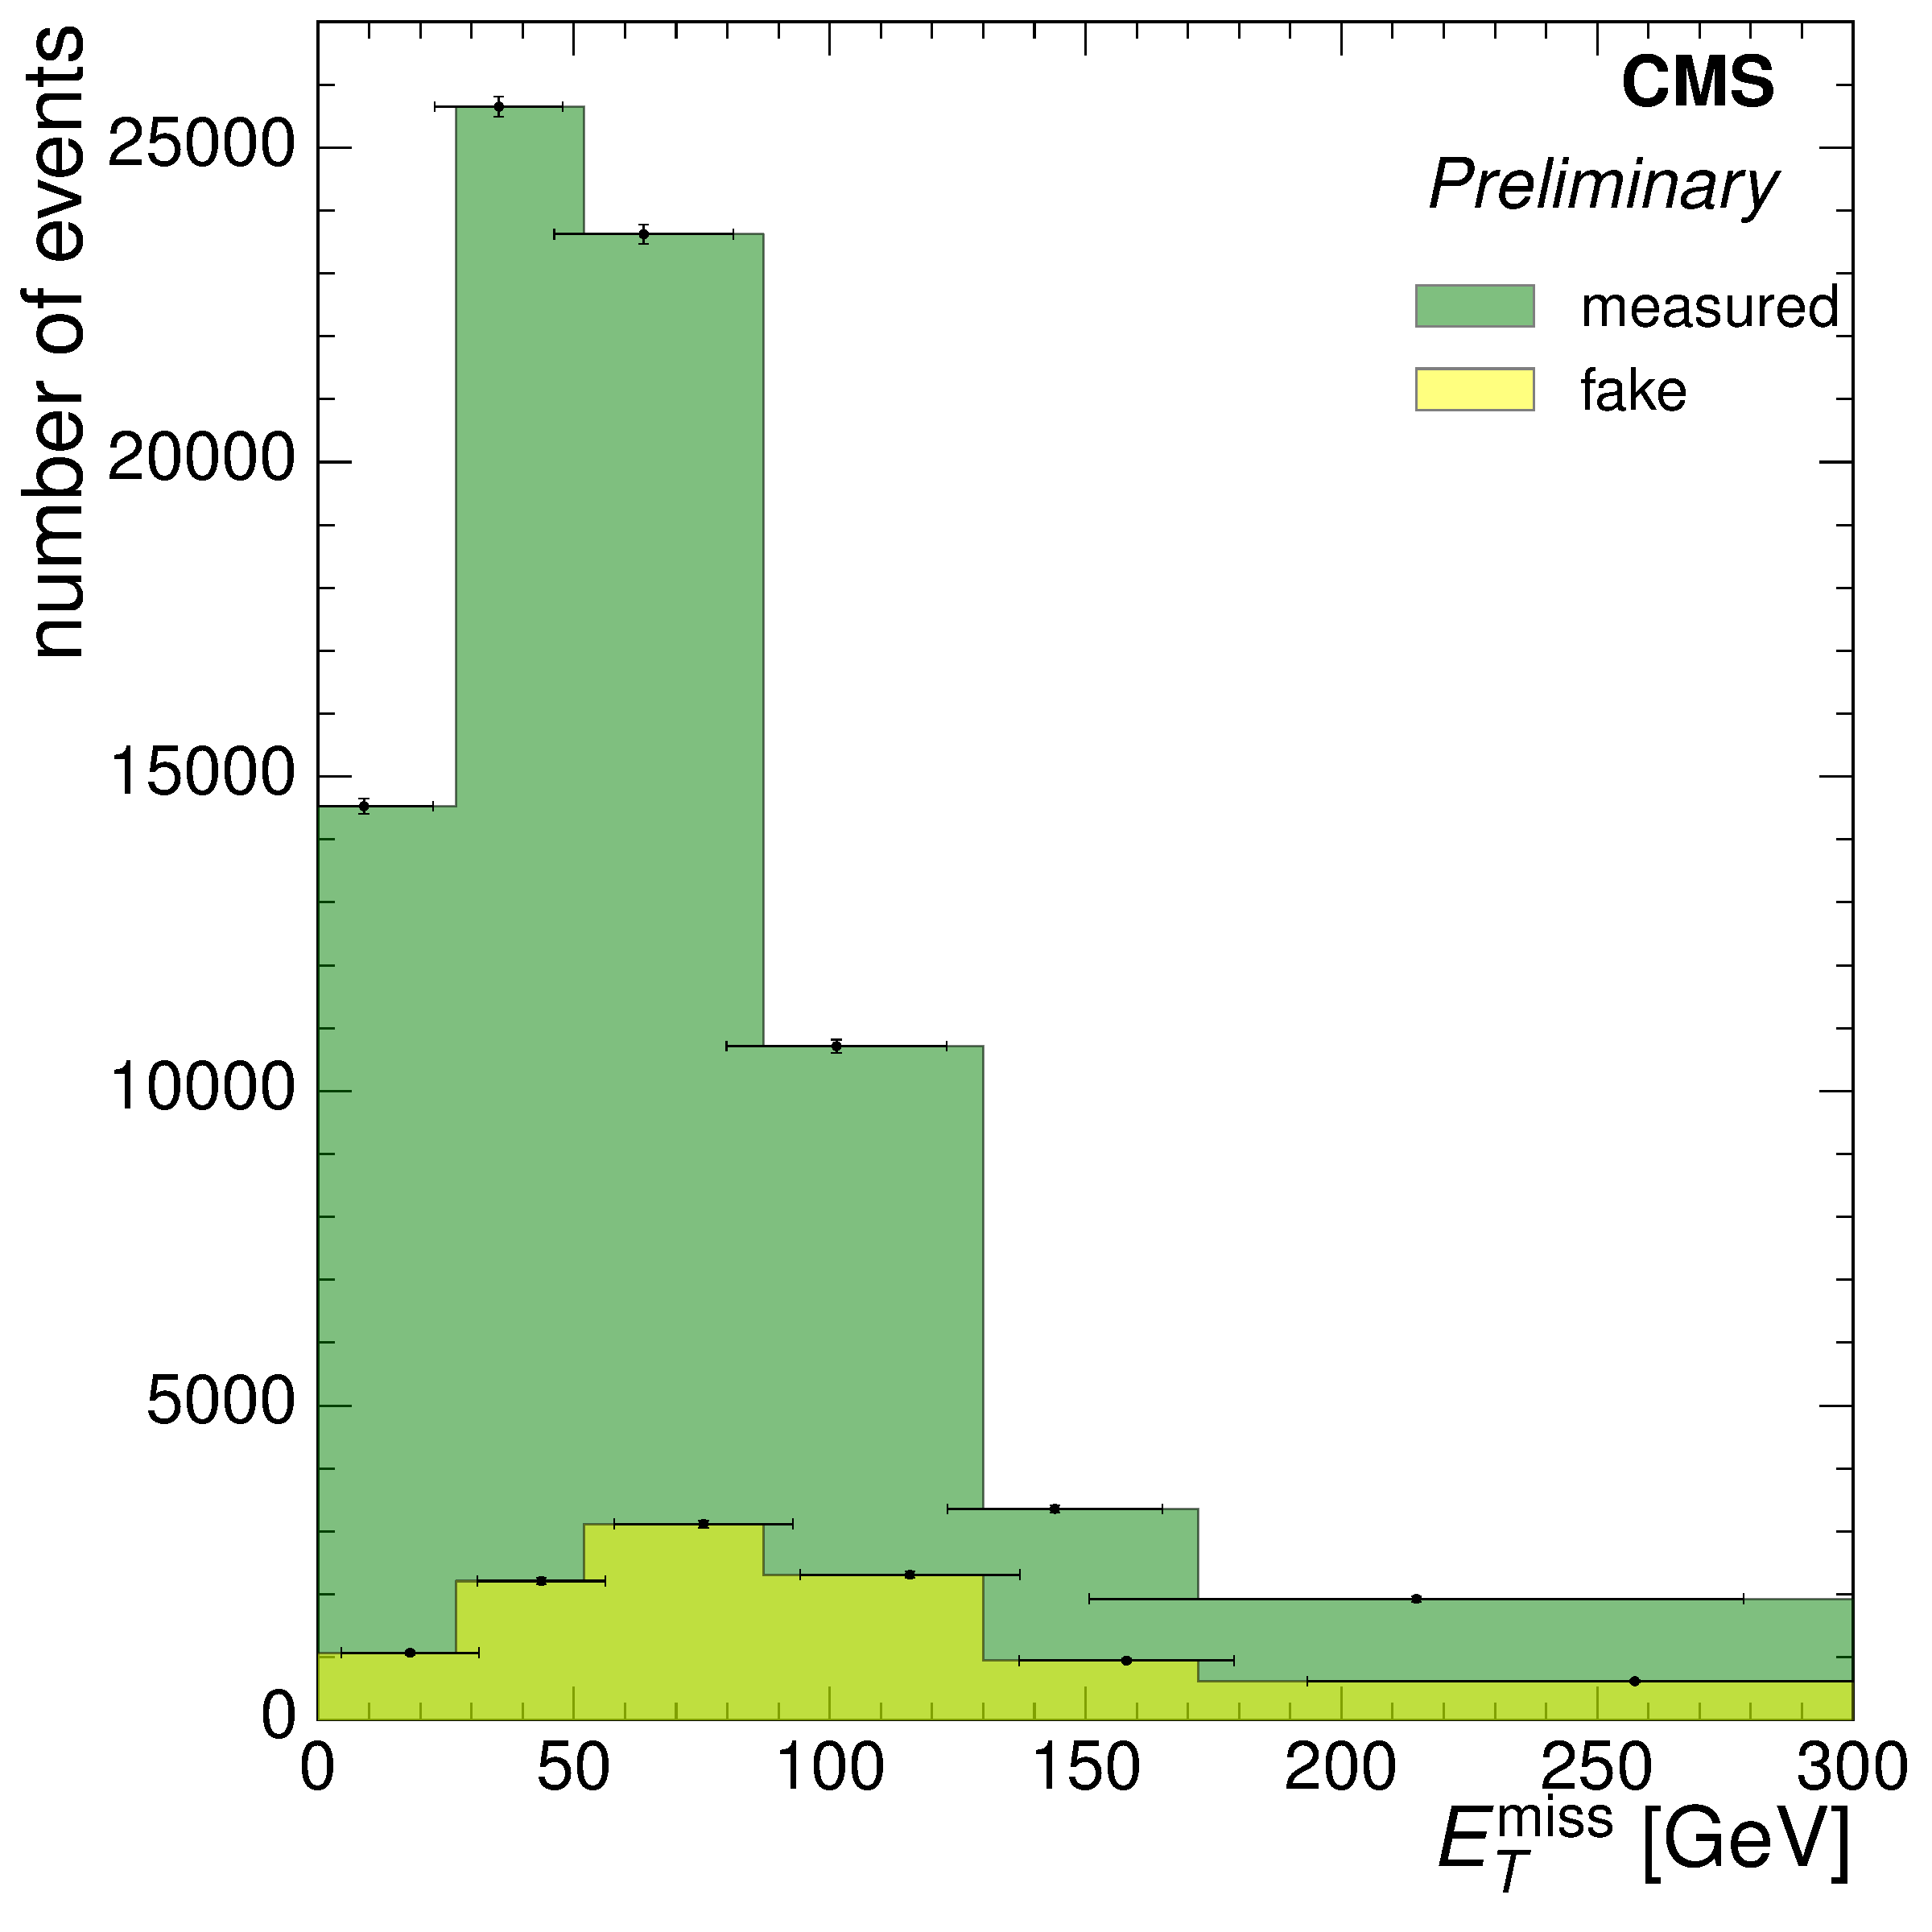
\includegraphics[width=0.48\textwidth]{Chapters/04_Analysis/04b_XSections/images/tau_cross_checks/comparison_measured_fake_TTJets_normalised_to_nevents.pdf}
     \caption[Comparison of the signal and fake distributions in the \met variable from semi-leptonic \ttbar
	 events in the electron+jets channel at $\roots=8\TeV$.]{Comparison of the signal and fake distributions from
	 semi-leptonic \ttbar events after selection in simulation in the electron+jets channel at $\roots=8\TeV$
	 normalised to one (left) and normalised to the numbers of events (right).}
     \label{fig:tau_shape_number_comparison}
\end{figure}

The difference between the tau energy down ($-1\sigma$) variation and the nominal measurements in the \met
variable before fitting and unfolding is shown in Figure~\ref{fig:tau_down_comparison}. In the highest \met
bin, the difference is approximately 6\%, and this value remains approximately constant after fitting and
unfolding. %, as shown in Table~\ref{tab:tau_up_down_final_bin_comparison}.
The significant affect of varying the tau energy is therefore unlikely to be an artifact of the fitting and/or
unfolding procedure, but a real difference in the number of events.

\begin{figure}[hbtp]
    \centering
     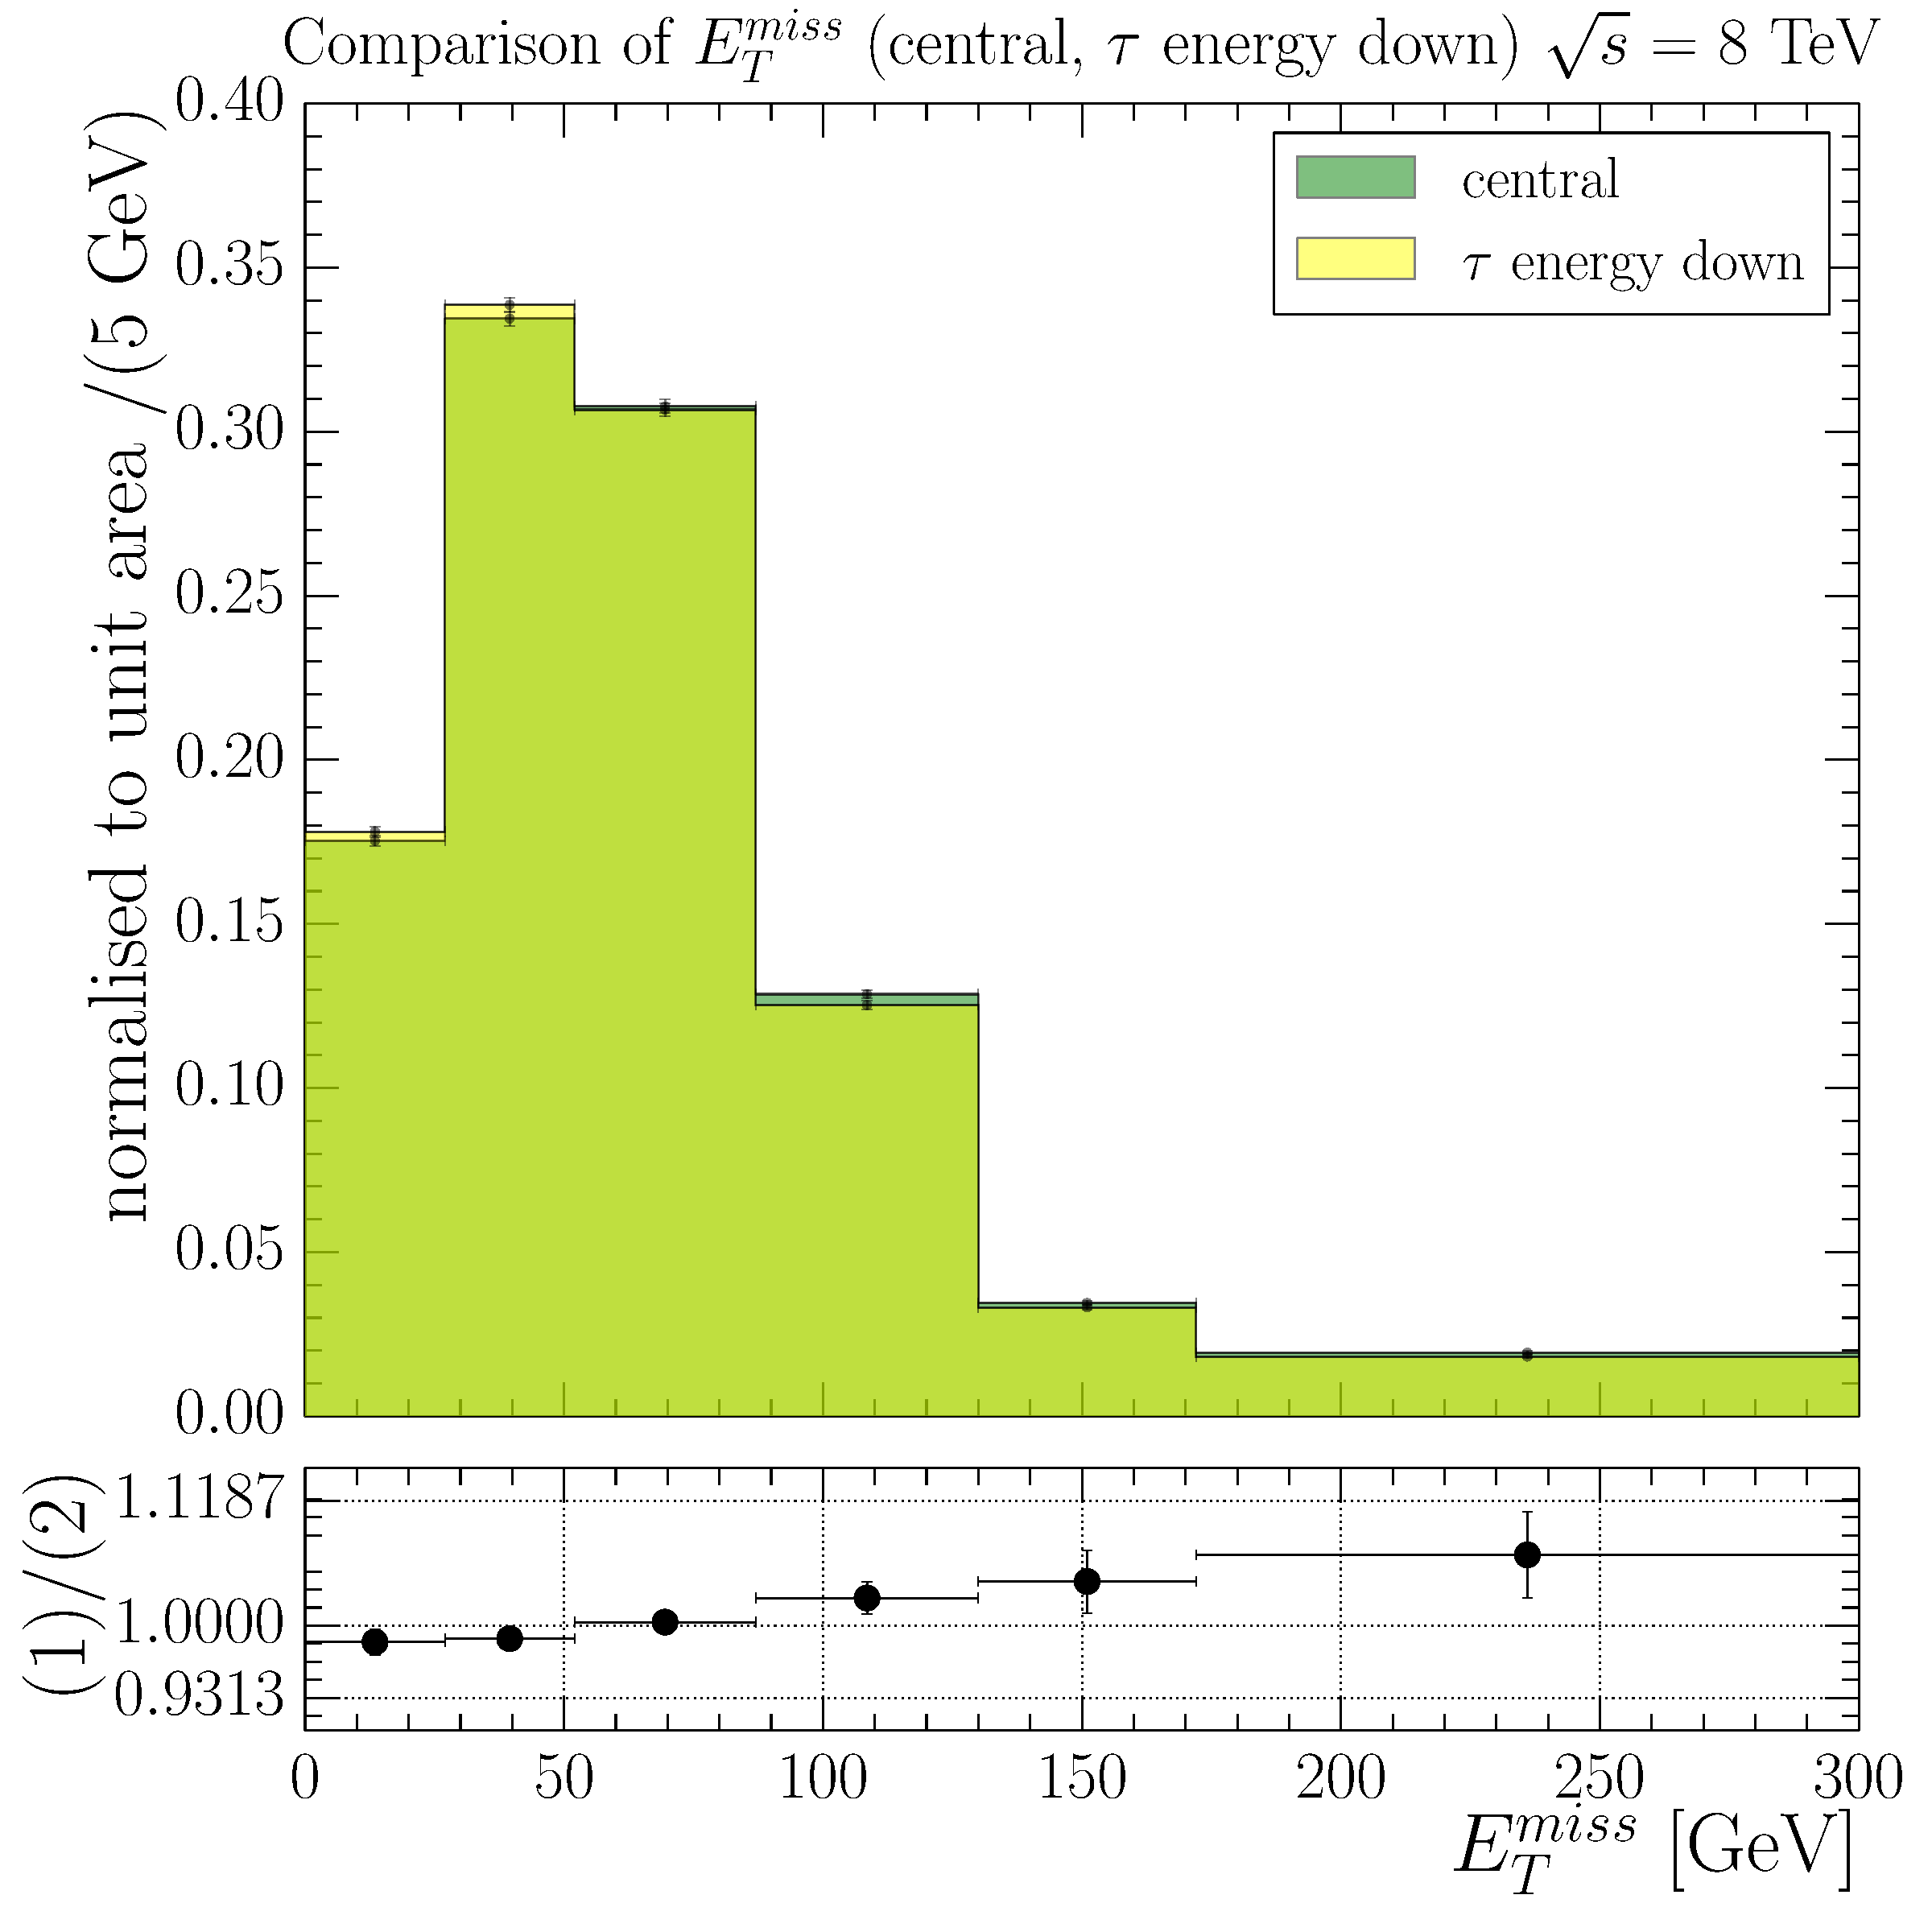
\includegraphics[width=0.48\textwidth]{Chapters/04_Analysis/04b_XSections/images/tau_cross_checks/compare_central_MET_to_tau_energy_down_asym_bins_electron_channel_data.pdf}\hfill
     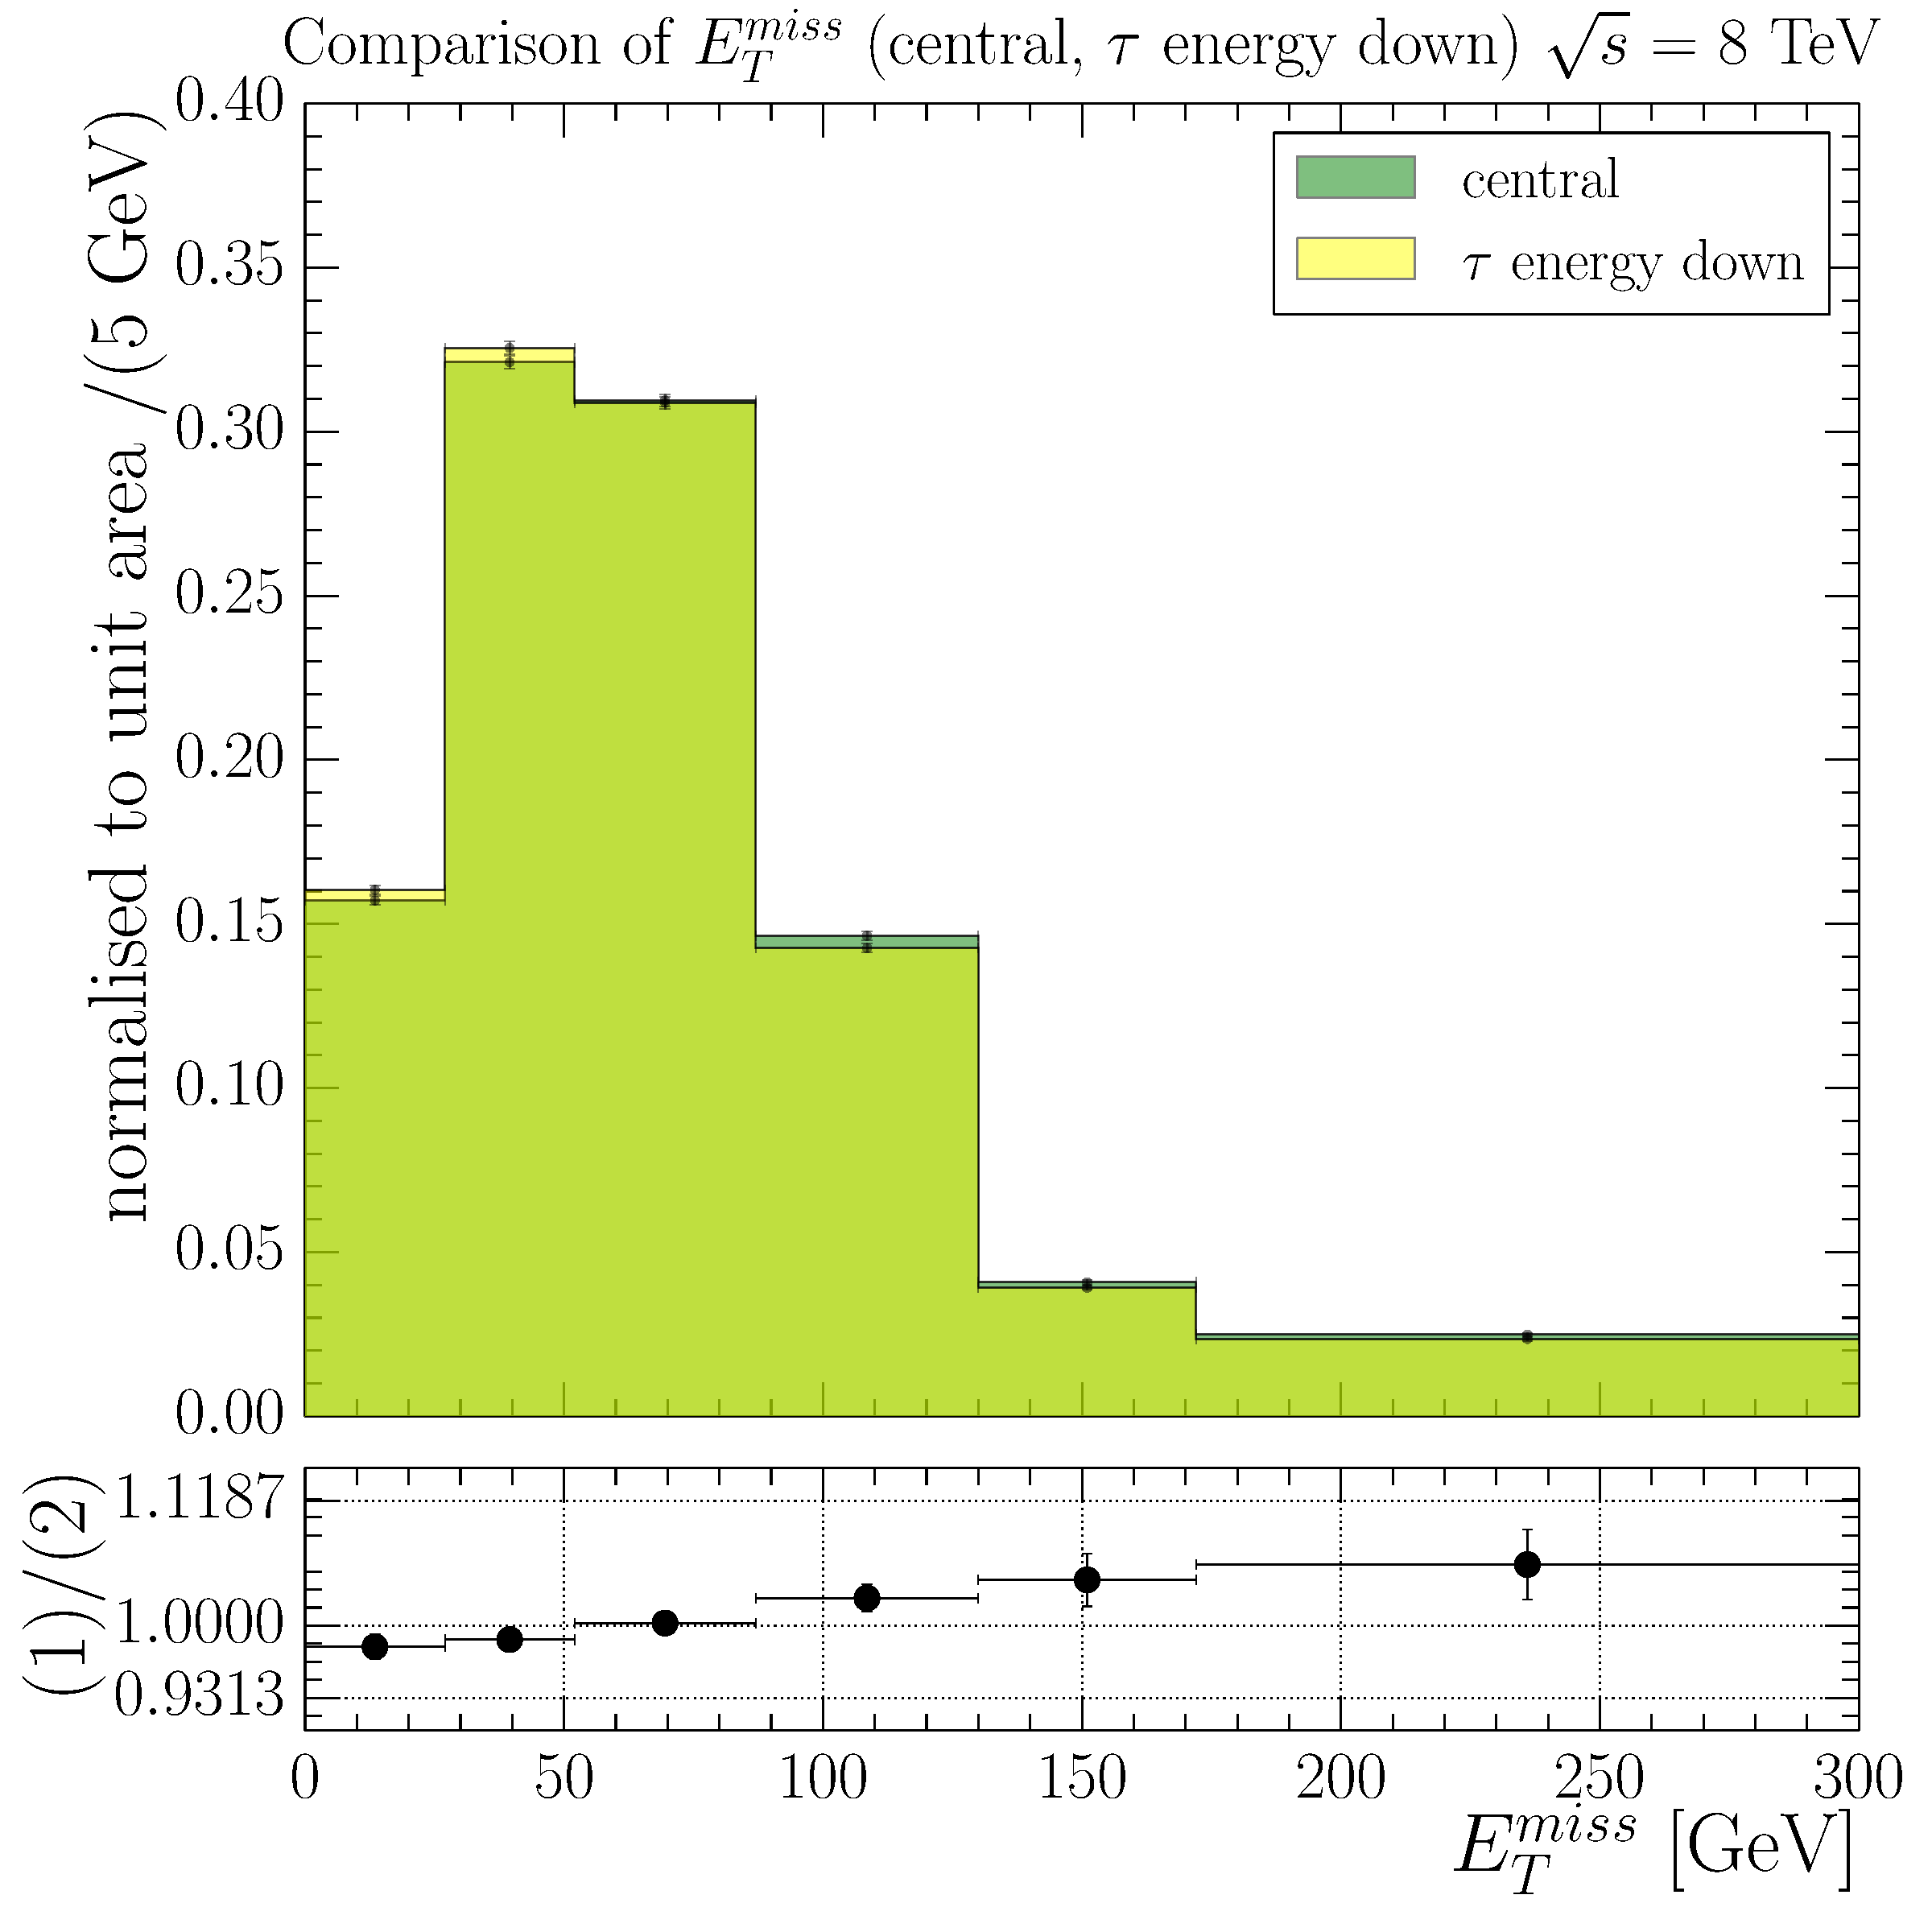
\includegraphics[width=0.48\textwidth]{Chapters/04_Analysis/04b_XSections/images/tau_cross_checks/compare_central_MET_to_tau_energy_down_asym_bins_electron_channel_TTJet.pdf}
     \caption[Comparison of the \met distributions in the nominal measurement and in the tau energy down
     variation in data and in simulation.]{Comparison of the \met distributions in the nominal measurement and
     in the tau energy down variation before fitting and unfolding in data (left) and in \ttbar simulation
     (right) at $\roots=8\TeV$}
     \label{fig:tau_down_comparison}
\end{figure}
 
%%% ============================================================
% Difference between central and tau energy up and down systematic value in highest \met bin
%% ============================================================
\begin{table}[htbp]
\centering
\caption{Difference between central and tau energy up and down systematic value in highest \met bin at a
centre-of-mass energy of 8 TeV in the electron channel TODO: FILL TABLE} %TODO: FILL TABLE
\label{tab:tau_up_down_final_bin_comparison}
\resizebox{\columnwidth}{!} {
\begin{tabular}{lrr}
\hline
Stage & $\tau$ energy up & $\tau$ energy down \\
\hline
Before Fitting \& Unfolding(\%) & & \\
After Fitting, before Unfolding(\%) & & \\
After Fitting \& Unfolding(\%) & & \\
\hline
\end{tabular}
}
\end{table}


Other small sources of experimental uncertainty include the non-clustered energy uncertainty (which refers to
fluctuations in deposits in the electromagnetic calorimeter that are not included in jet clusters), the
matching threshold and factorisation and normalisation scale uncertainties in \WpJets and \ZpJets events,
pileup uncertainty, the QCD template shape uncertainty, and the efficiency of electron, muon and \btagging in
the selection process.

Rate changing systematics such as the uncertainty on the luminosity and the uncertainty on the theoretical
cross sections of the signal and background processes have a negligible effect on the final result, since
they cance in the final normalised measurements.

\subsection{Theoretical Uncertainties}
\label{ss:theoretical_uncertainties}

\subsubsection{7~\TeV V+Jets theory systematic template}
\label{sss:7TeV_vjets_theory_systematic_template}

The factorisation and normalisation scale ($Q^{2}$ up/down) uncertainty is evaluated using simulation samples
produced with the scale varied by factors of 2 (up) and 0.5 (down). This has been evaluated to be one of the
dominating uncertainties in this analysis. The uncertainty in the matching theshold (matching up/down) for
\ttbar events is evaluated in the same way.

Unfortunately, Monte Carlo simulation for theoretical systematic uncertainties at $\roots=7\TeV$ have not
been made available for W+jets and Z+jets processes. However, it can be seen in
Figure~\ref{fig:wjets_7TeV_8TeV_comparison} that the W+jets template shapes at $\roots=7\TeV$ and
$\roots=8\TeV$ are similar. The V+jets template shapes used to evaluate these theoretical systematics are
therefore obtained from $\roots=8\TeV$ theoretical systematic datasets, and then scaled to the normalisation
in the nominal sample at $\roots=7\TeV$.

\begin{figure}[hbtp]
    \centering
     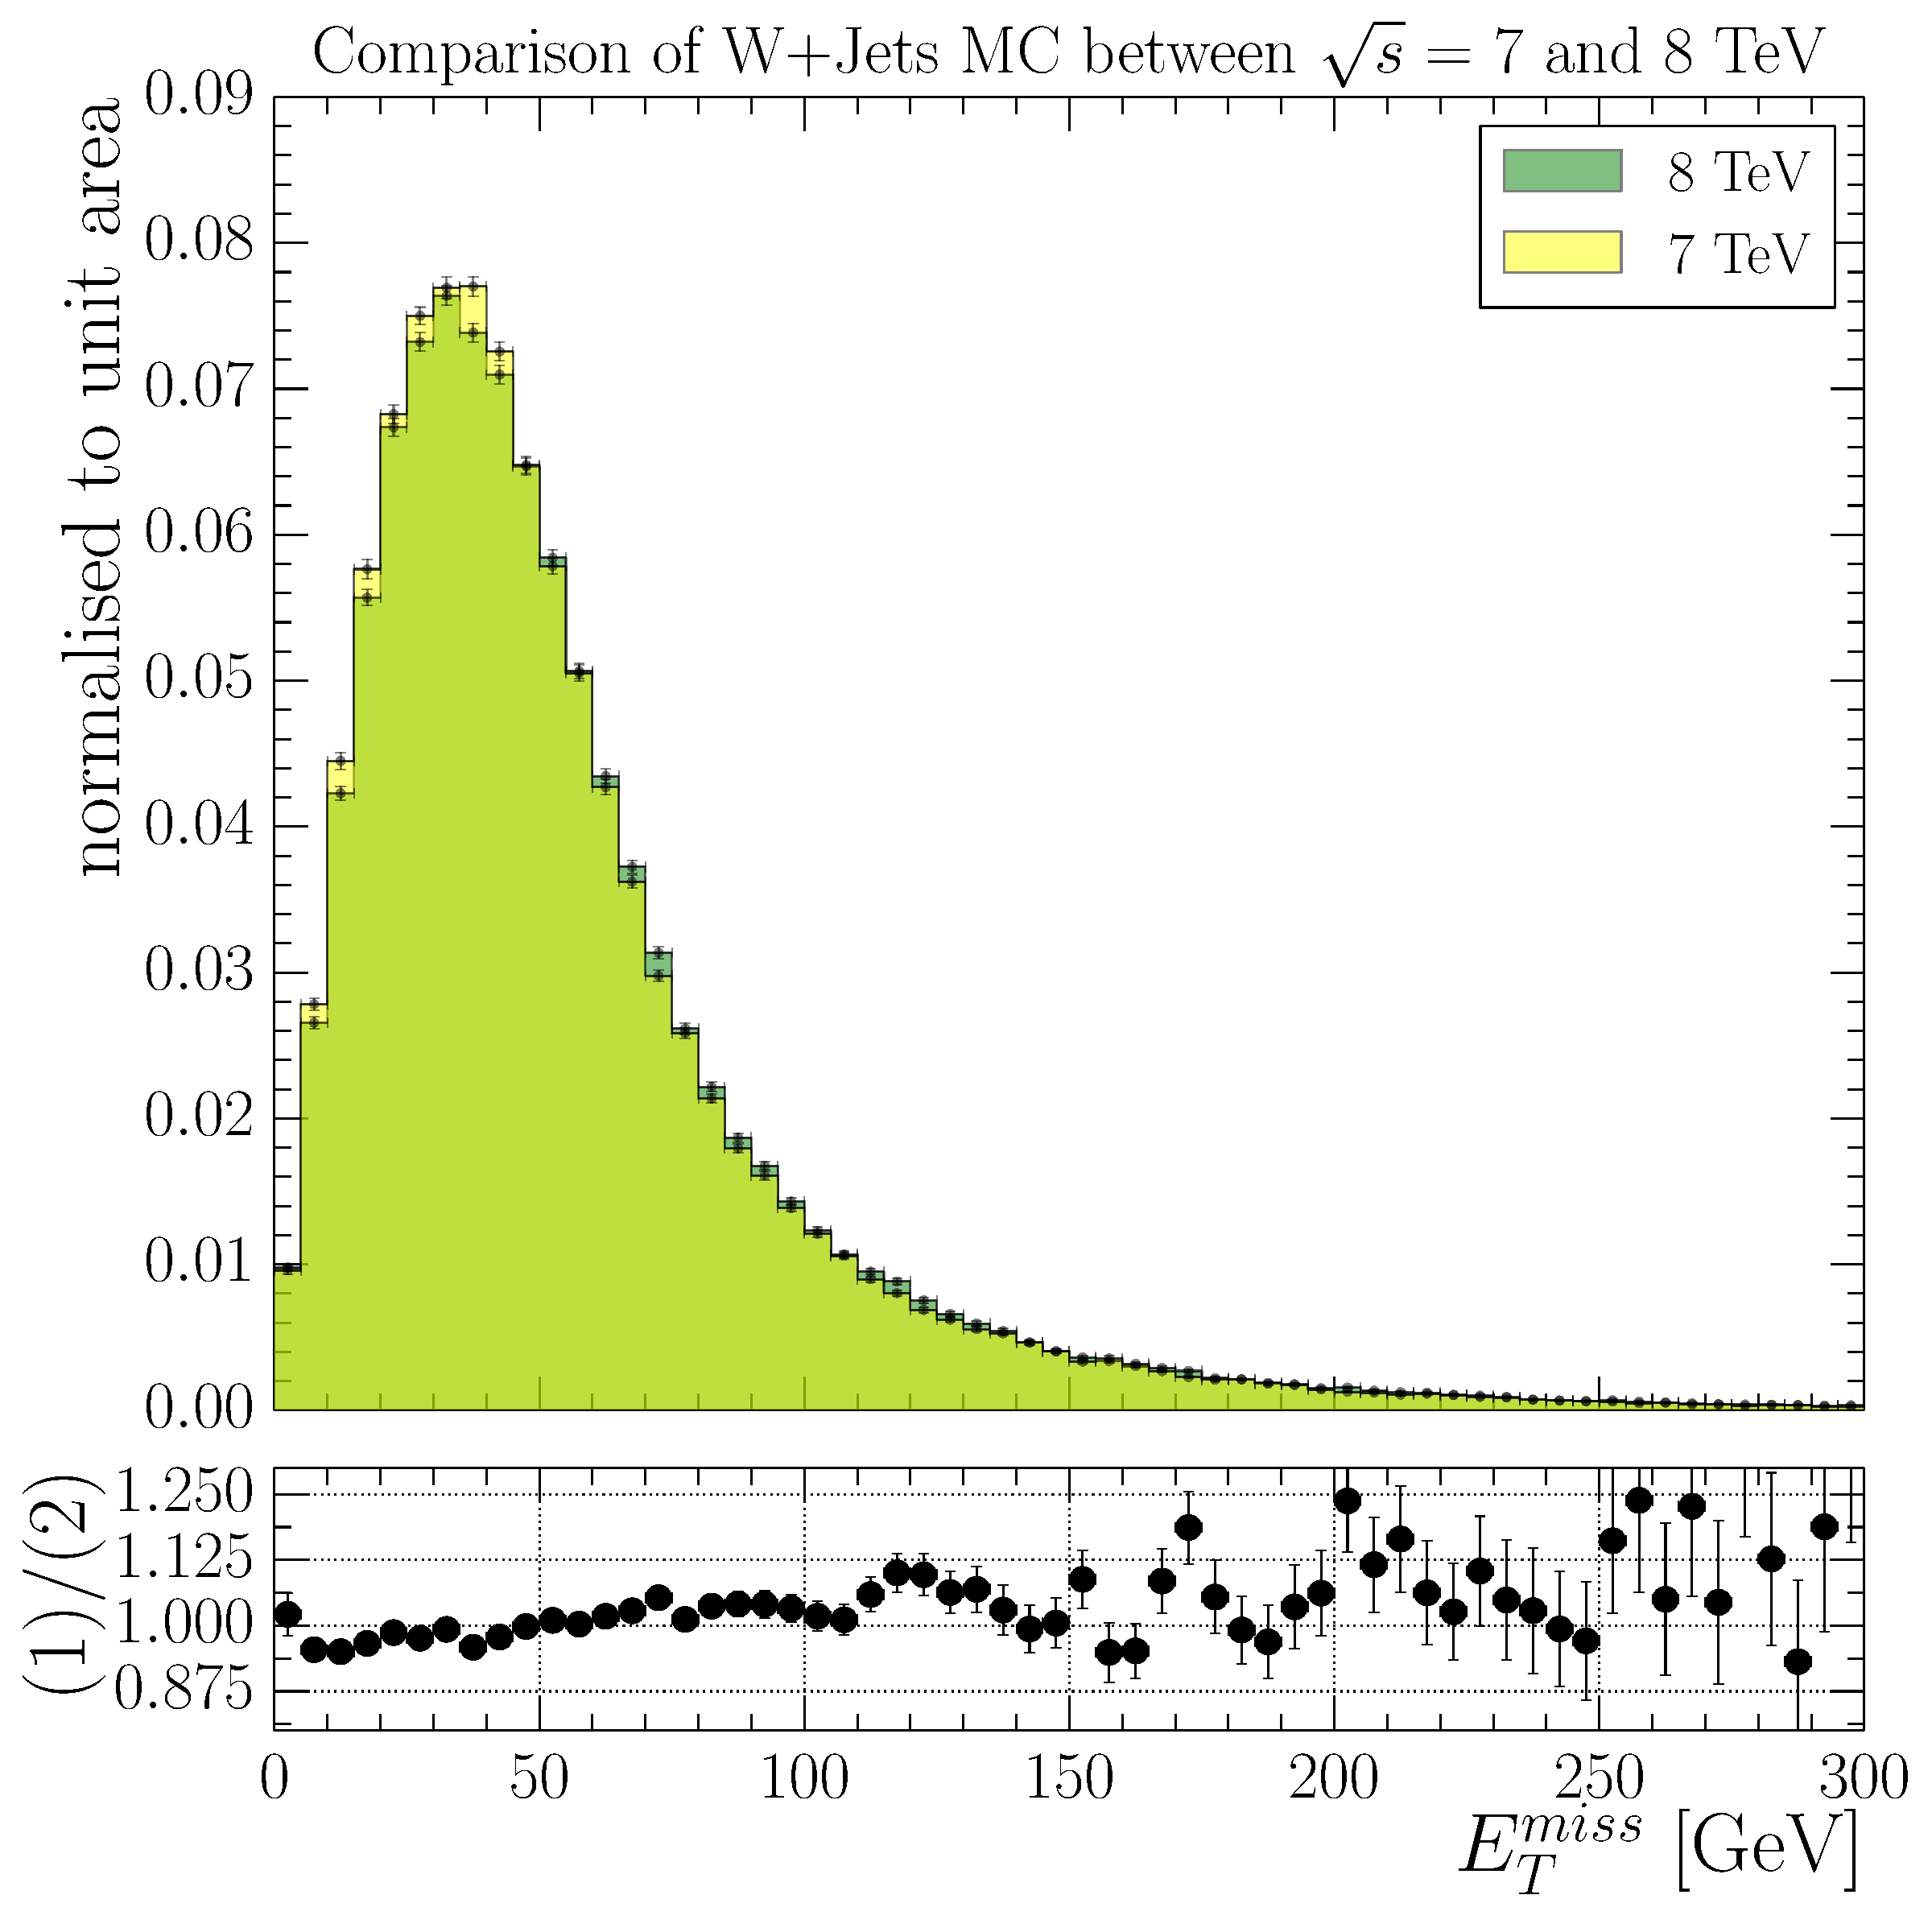
\includegraphics[width=0.48\textwidth]{Chapters/04_Analysis/04b_XSections/images/WJets_comparison/TTbar_plus_X_analysis_EPlusJets_Refselection_MET_patType1CorrectedPFMet_MET_0orMoreBtag.pdf}\hfill
     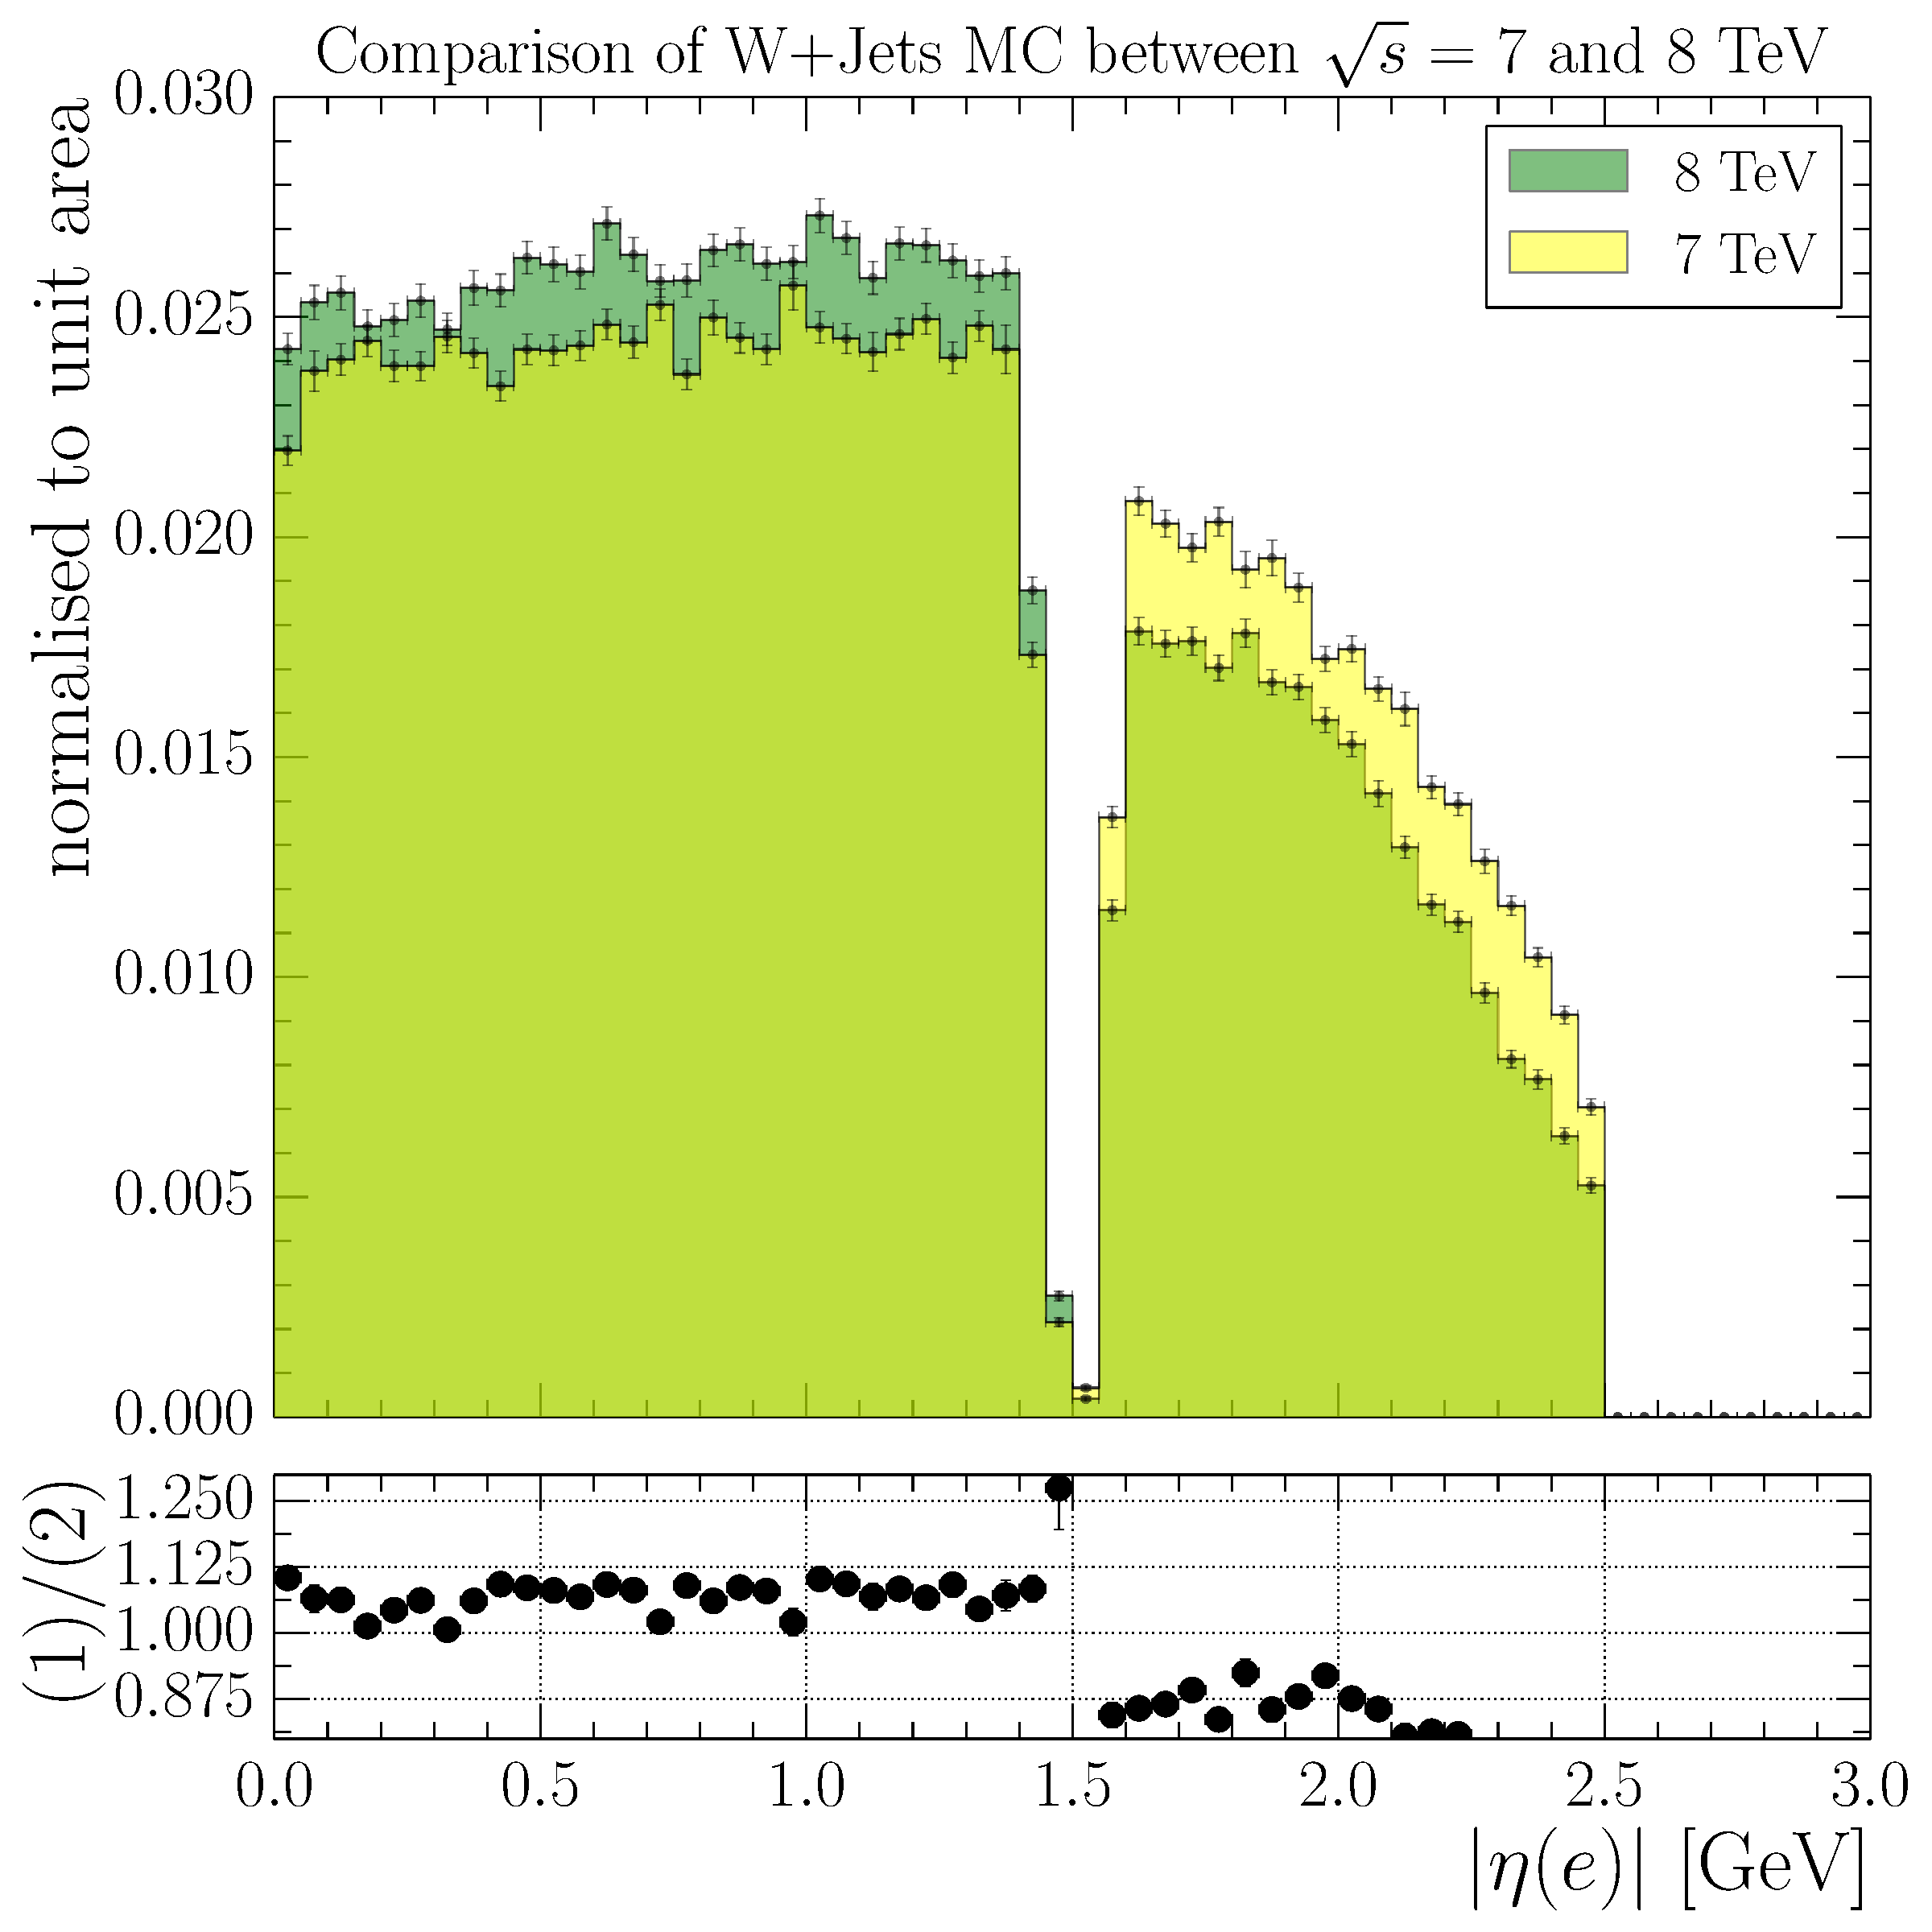
\includegraphics[width=0.48\textwidth]{Chapters/04_Analysis/04b_XSections/images/WJets_comparison/TTbar_plus_X_analysis_EPlusJets_Refselection_Electron_electron_AbsEta_0orMoreBtag.pdf}\\
	 \caption[\met and electron \abseta shape comparison of W+jets templates in $\roots=7\TeV$ and
	 $\roots=8\TeV$ in the electron+jets channel.]{Shape comparison of W+jets templates in $\roots=7\TeV$ and
	 $\roots=8\TeV$ Monte Carlo simulation for \met (left) and electron \abseta (right) in the electron+jets
	 channel.}
     \label{fig:wjets_7TeV_8TeV_comparison}
\end{figure}

\subsubsection{Hadronisation Uncertainty}
\label{sss:hadronisation_uncertainty}
The uncertainty due to hadronisation modelling is evaluated by comparing a simulated sample
generated using the \POWHEG generator and \PYTHIA to model the hadron showering (\POWHEG+ \PYTHIA) to a sample
generator using the same \POWHEG generator and \HERWIG to model the hadron showering (\POWHEG+ \HERWIG). The
difference between the \PYTHIA and \HERWIG samples is scaled to the nominal measurement and taken as the
hadronisation uncertainty. All variables, and in particular those sensitive to hadronic aspects of an event
such as \HT and \st, are significantly affected by this systematic, with a larger uncertainty in lower bins of
the primary variables.

\subsubsection{PDF Uncertainties}
\label{sss:PDF_uncertainties}
The proton PDF uncertainties are evaluated similarly, with 44 distinct weights from the CTEQ 6.6 PDF sets used
to reweight events in the simulated samples and repeat the analysis.
The top quark mass uncertainty is evaluated using \ttbar samples produced with two different top quark masses
of 169.5\GeV and 173.5\GeV, and scaling the the error obtained using these samples to the top mass uncertainty of
$\pm1.0\GeV$.

\subsubsection{\ttbar \pt Mismodelling}
\label{sss:top_pt_modelling}
There is a known issue with event generators mismodelling the top quark \pt distribution; the distribution of
the transverse momentum of top quarks in data was found to be softer than that in simulation
\cite{Chatrchyan:2012saa}. Scale factors have been derived to correct for this disagreement. The effect of
this correction on the nominal measurement was evaluated to be negligible for low values of the primary
variables, increasing to 3--7\% at higher values. The \MADGRAPH simulation after applying the \tquark \pt
correction is also included in the results plots (Figures~\ref{fig:result_MET_HT_ST_7TeV_combined} to
\ref{fig:result_WPT_MT_8TeV_combined}), but this is not included as a systematic error.

The most significant shape changing uncertainties typically arise from the factorisation scale variations in
the \ttbar process and the hadronisation.

\subsection{Systematic Uncertainty Tables}
\label{ss:systematic_uncertainty_tables}

Tables~\ref{tab:typical_systematics_7TeV_combined} and \ref{tab:typical_systematics_8TeV_combined} give
typical (median) relative systematic uncertainties for all systematic uncertainty sources, at $\roots=7\TeV$
and $\roots=8\TeV$ respectively, and are for the combined electron+jets and muon+jets channel, for the fitting
method. The sources are grouped into categories, taking only the maximum relative uncertainty between a
$+1\sigma/-1\sigma$ variation of each uncertainty source. In categories containing more than one
$+1\sigma/-1\sigma$ variation pair (\met uncertanties: electron/muon/tau/unclustered energy; Background
(other):\ttbar/single top/\VpJets/QCD cross sections and luminosity; Theoretical Systematics: \ttbar/\VpJets
matching and $Q^{2}$), the maximum uncertainty of each $+1\sigma/-1\sigma$ source is added in quadrature. The
median values across all of the bins of a primary variable are then taken as the typical systematic
uncertainties stated in the tables. Extended uncertainty tables can be found in
Appendix~\ref{as:systematic_uncertainties}.

%% ============================================================
% Typical systematics table for combined channel, k-value None, met type patType1CorrectedPFMet, 2orMoreBtags b-tag region
%% ============================================================
\begin{table}[htbp]
\centering
\caption{Typical systematic uncertainties in percent (median values) for the normalised \ttbar
differential cross section measurement at $\roots=7\TeV$ (combination of electron and muon channels). Typical
values of the total systematic uncertainty are also shown.}
\label{tab:typical_systematics_7TeV_combined}
\resizebox{\columnwidth}{!} {
\begin{tabular}{lrrrrr}
\hline
Uncertainty source & \met & \HT &  \st & \wpt & \mt \\
\hline
Electron trigger and selection efficiencies & $<1$ & 1.30 & 1.41 & $<1$ & $<1$ \\
Muon trigger and selection efficiencies & $<1$ & $<1$ & $<1$ & $<1$ & $<1$ \\
\btagging & $<1$ & $<1$ & 2.1 & $<1$ & $<1$ \\
Jet Energy Scale & $<1$ & 3.6 & 1.1 & $<1$ & $<1$ \\
Jet Energy Resolution & $<1$ & 3.1 & 1.6 & $<1$ & $<1$ \\
\met uncertainties & 1.3 & - & 2.6 & 4.3 & $<1$ \\
Pileup & $<1$ & 0.1 & 2.4 & $<1$ & $<1$ \\
QCD shape & $<1$ & $<1$ & 2.2 & $<1$ & $<1$ \\
Background (other) & $<1$ & $<1$ & 4.1 & $<1$ & $<1$ \\
Theoretical systematics & 1.0 & 4.6 & 4.7 & $<1$ & 1.0 \\
top mass & $<1$ & $<1$ & $<1$ & $<1$ & $<1$ \\
hadronisation & 2.1 & 9.9 & 8.2 & 3.8 & 1.1 \\
PDF uncertainties & $<1$ & $<1$ & $<1$ & $<1$ & $<1$ \\
\pt reweighting & 1.6 & $<1$ & 1.3 & $<1$ & $<1$ \\
\hline
Total & 3.7 & 12.4 & 13.3 & 6.6 & 2.9 \\
\hline 
\end{tabular}
}
\end{table}

%Jet Energy Resolution (\%) & 0.07& 0.07& 0.07& 3.11& 1.58& 0.21& 0.44 
%Jet Energy Scale (\%) & 0.22& 0.22& 0.22& 3.55& 1.13& 0.50& 0.90 
%$E_{T}^{miss}$ uncertainties (\%) & 1.28& 1.28& 1.28& -& 2.57& 0.96& 4.31 
%PDF uncertainties (\%) & 0.66& 0.66& 0.66& 0.79& 0.88& 0.82& 0.96 
%pileup (\%) & 0.05& 0.05& 0.05& 0.12& 2.40& 0.11& 0.65 
%QCD shape (\%) & 0.02& 0.02& 0.02& 0.16& 2.23& 0.06& 0.05 
%Background (other) (\%) & 0.00& 0.00& 0.00& 0.02& 3.61& 0.00& 0.38 
%btagging (\%) & 0.03& 0.03& 0.03& 0.04& 2.09& 0.03& 0.23 
%Electron trigger efficiency \& electron selection (\%) & 0.01& 0.01& 0.01& 1.30& 1.41& 0.27& 0.85 
%hadronisation (\%) & 2.06& 2.06& 2.06& 9.91& 8.22& 1.10& 3.75 
%Muon trigger efficiency \& muon selection (\%) & 0.00& 0.00& 0.00& 0.02& 0.00& 0.01& 0.01 
%$p_\mathrm{T}$ reweighting (\%) & 1.63& 1.63& 1.63& 0.80& 1.25& 0.55& 0.21 
%Theoretical systematics (\%) & 1.01& 1.01& 1.01& 4.55& 4.67& 1.00& 0.84 
%top mass (\%) & 0.19& 0.19& 0.19& 0.29& 0.41& 0.21& 0.29 


%% ============================================================
% Typical systematics table for combined channel, k-value None, met type patType1CorrectedPFMet, 2orMoreBtags b-tag region
%% ============================================================
\begin{table}[htbp]
\centering
\caption{Typical systematic uncertainties in percent (median values) for the normalised \ttbar
differential cross section measurement at $\roots=8\TeV$ (combination of electron and muon channels). Typical
values of the total systematic uncertainty are also shown.}
\label{tab:typical_systematics_8TeV_combined}
\resizebox{\columnwidth}{!} {
\begin{tabular}{lrrrrr}
\hline
Uncertainty source & \met & \HT &  \st & \wpt & \mt \\
\hline
Electron trigger and selection efficiencies & $<1$ & $<1$ & $<1$ & $<1$ & $<1$ \\ 
Muon trigger and selection efficiencies & $<1$ & $<1$ & $<1$ & $<1$ & $<1$ \\  
\btagging & $<1$ & $<1$ & $<1$ & $<1$ & $<1$ \\
Jet Energy Scale & $<1$ & 1.7 & 1.4 & 0.5 & 0.7 \\ 
Jet Energy Resolution & $<1$ & $<1$ & $<1$ & $<1$ & $<1$ \\
\met uncertainties & 2.8 & - & 1.0 & 2.4 & $<1$ \\
Pileup & $<1$ & $<1$ & $<1$ & $<1$ & $<1$ \\
QCD shape & $<1$ & $<1$ & $<1$ & $<1$ & $<1$ \\
Background (other) & $<1$ & $<1$ & $<1$ & $<1$ & $<1$ \\
Theoretical systematics & 7.2 & 5.2 & 3.7 & 3.2 & 1.7 \\
Top quark mass & $<1$ & $<1$ & $<1$ & $<1$ & $<1$ \\
Hadronisation & 4.2 & 4.6 & 7.2 & 3.0 & 1.4 \\
PDF uncertainties & $<1$ & $<1$ & $<1$ & $<1$ & $<1$ \\
\pt reweighting & $<1$ & $<1$ & $<1$ & $<1$ & $<1$ \\
\hline 
Total & 9.6 & 14.1 & 12.54 & 9.46 & 2.86 \\
\hline
\end{tabular}
}
\end{table}


%Jet Energy Resolution (\%) & 0.22& 0.43& 0.23& 0.26& 0.59 
%Jet Energy Scale (\%) & 0.77& 1.68& 0.49& 0.70& 1.38 
%$E_{T}^{miss}$ uncertainties (\%) & 2.80& -& 2.42& 0.72& 1.04 
%PDF uncertainties (\%) & 0.50& 0.50& 0.48& 0.15& 0.52 
%pileup (\%) & 0.22& 0.39& 0.58& 0.23& 0.10 
%QCD shape (\%) & 0.11& 0.24& 0.15& 0.28& 0.14 
%Background (other) (\%) & 0.00& 0.00& 0.01& 0.00& 0.02 
%btagging (\%) & 0.21& 0.02& 0.11& 0.01& 0.10 
%Electron trigger efficiency \& electron selection (\%) & 0.20& 0.12& 0.62& 0.07& 0.02 
%hadronisation (\%) & 4.23& 4.56& 3.06& 1.44& 7.15 
%Muon trigger efficiency \& muon selection (\%) & 0.01& 0.02& 0.02& 0.01& 0.01 
%$p_\mathrm{T}$ reweighting (\%) & 0.83& 0.78& 0.40& 0.73& 0.53 
%Theoretical systematics (\%) & 7.19& 5.15& 3.16& 1.67& 3.73 
%top mass (\%) & 0.33& 0.93& 0.54& 0.10& 0.72 


\section{Results}
\label{s:results}

The fitting and unfolding explained in Sections~\ref{s:maximum_likelihood_fit} and \ref{ss:unfolding} is
performed individually in the electron+jets and muon+jets channels, resulting in a number of \ttbar events in
each channel. The measurement is then carried out as outlined in Section~\ref{ss:measurement} on the numbers
of events in each channel, in addition to the sum total of the two channels to calculate the cross section in
the combined semi-leptonic channel. This section summarises the normalised differential cross sections for the
primary variables investigated in this analysis. Figures~\ref{fig:result_MET_HT_ST_7TeV_combined}
and \ref{fig:result_WPT_MT_7TeV_combined} show the distributions at $\roots=7\TeV$; and
Figures~\ref{fig:result_MET_HT_ST_8TeV_combined} and \ref{fig:result_WPT_MT_8TeV_combined} show the
distributions at $\roots=8\TeV$. Corresponding numerical results are included in Appendix~\ref{as:results}.
Results plots showing the unfolded data distributions from the background subtraction method of extracting the
\ttbar event yield are also shown in Appendix~\ref{as:results}.

The normalised cross section distributions are shown compared with predictions from \MADGRAPH,
\POWHEG+\PYTHIA, \POWHEG+\HERWIG, \MCATNLO ($\roots=8\TeV$ only) and a \MADGRAPH prediction with corrected
\tquark \pt in the left hand plots. The error bars on the data points represent the statistical +unfolding
(inner) and systematic uncertainties summed in qudrature (outer). In the right hand plots a comparison with
the \MADGRAPH prediction with matching threshold, and factorisation and renormalisation scale up and down.
Ratio plots are shown below the distribution plots to allow easier comparison of the distribution in data to
the different simulations, with a line at 1.0 for reference. In the ratio plots, the grey error bands
represent the statistical + unfolding uncertainty, while the yellow error bands represent the systematic
uncertainties added in qudrature. The systematic uncertainties resulting from matching and factorisation and
renormalisation scale are excluded from the systematic uncertainties in plots comparing the data distribution
with theoretical variations. Similarly, the hadronisation uncertainty is excluded in plots comparing the data
distribution with different simulation generators. It can be seen that the data distributions show softer
distributions than in simulation as a result of the mismodelling of the \tquark \pt in the generators
\cite{Chatrchyan:2012saa}. The corrected \MADGRAPH distribution, however, shows good agreement with the data.

\begin{figure}[hbtp]
    \centering
%     \resizebox{\columnwidth}{!} {
     \includegraphics[width=0.48\textwidth]{Chapters/04_Analysis/04b_XSections/images/results/fit/7TeV/MET/central/normalised_xsection_combined_different_generators.pdf}\hfill
     \includegraphics[width=0.48\textwidth]{Chapters/04_Analysis/04b_XSections/images/results/fit/7TeV/MET/central/normalised_xsection_combined_systematics_shifts.pdf}\\
     \includegraphics[width=0.48\textwidth]{Chapters/04_Analysis/04b_XSections/images/results/fit/7TeV/HT/central/normalised_xsection_combined_different_generators.pdf}\hfill
     \includegraphics[width=0.48\textwidth]{Chapters/04_Analysis/04b_XSections/images/results/fit/7TeV/HT/central/normalised_xsection_combined_systematics_shifts.pdf}\\
     \includegraphics[width=0.48\textwidth]{Chapters/04_Analysis/04b_XSections/images/results/fit/7TeV/ST/central/normalised_xsection_combined_different_generators.pdf}\hfill
     \includegraphics[width=0.48\textwidth]{Chapters/04_Analysis/04b_XSections/images/results/fit/7TeV/ST/central/normalised_xsection_combined_systematics_shifts.pdf}\\
     \caption[Comparison of the measured normalised differential cross section with respect to \met, \HT and
     \st to different Monte Carlo generators and predictions at $\roots=7\TeV$.]{Comparison of the measured
     normalised differential cross section with respect to \met (upper), \HT (middle) and \st (lower) to
     different Monte Carlo generators: \MADGRAPH, \POWHEG+\HERWIG, \POWHEG+\PYTHIA and \MADGRAPH corrected for
     top \pt mismodelling (left) and to different Monte Carlo predictions matching threshold up/down and
     factorisation scale up/down (right) in the combined electron+jets and muon+jets channel at
     $\roots=7\TeV$. The lower plots show the ratio of the predictions to the data.}
     \label{fig:result_MET_HT_ST_7TeV_combined}
 %    }
\end{figure}

\begin{figure}[hbtp]
    \centering
     \includegraphics[width=0.48\textwidth]{Chapters/04_Analysis/04b_XSections/images/results/fit/7TeV/WPT/central/normalised_xsection_combined_different_generators.pdf}\hfill
     \includegraphics[width=0.48\textwidth]{Chapters/04_Analysis/04b_XSections/images/results/fit/7TeV/WPT/central/normalised_xsection_combined_systematics_shifts.pdf}\hfill
     \includegraphics[width=0.48\textwidth]{Chapters/04_Analysis/04b_XSections/images/results/fit/7TeV/MT/central/normalised_xsection_combined_different_generators.pdf}\hfill
     \includegraphics[width=0.48\textwidth]{Chapters/04_Analysis/04b_XSections/images/results/fit/7TeV/MT/central/normalised_xsection_combined_systematics_shifts.pdf}\hfill
     \caption[Comparison of the measured normalised differential cross section with respect to \wpt and \mt to
     different Monte Carlo generators and predictions at $\roots=7\TeV$.]{Comparison of the measured
     normalised differential cross section with respect to \wpt and \mt to different Monte Carlo generators:
     \MADGRAPH, \POWHEG+\HERWIG, \POWHEG+\PYTHIA and \MADGRAPH corrected for top \pt mismodelling (left) and
     to different Monte Carlo predictions matching threshold up/down and factorisation scale up/down (right)
     in the combined electron+jets and muon+jets channel at $\roots=7\TeV$. The lower plots show the ratio of
     the predictions to the data.}
     \label{fig:result_WPT_MT_7TeV_combined}
\end{figure}


\begin{figure}[hbtp]
    \centering
     \includegraphics[width=0.48\textwidth]{Chapters/04_Analysis/04b_XSections/images/results/fit/8TeV/MET/central/normalised_xsection_combined_different_generators.pdf}\hfill
     \includegraphics[width=0.48\textwidth]{Chapters/04_Analysis/04b_XSections/images/results/fit/8TeV/MET/central/normalised_xsection_combined_systematics_shifts.pdf}\hfill
     \includegraphics[width=0.48\textwidth]{Chapters/04_Analysis/04b_XSections/images/results/fit/8TeV/HT/central/normalised_xsection_combined_different_generators.pdf}\hfill
     \includegraphics[width=0.48\textwidth]{Chapters/04_Analysis/04b_XSections/images/results/fit/8TeV/HT/central/normalised_xsection_combined_systematics_shifts.pdf}\hfill
     \includegraphics[width=0.48\textwidth]{Chapters/04_Analysis/04b_XSections/images/results/fit/8TeV/ST/central/normalised_xsection_combined_different_generators.pdf}\hfill
     \includegraphics[width=0.48\textwidth]{Chapters/04_Analysis/04b_XSections/images/results/fit/8TeV/ST/central/normalised_xsection_combined_systematics_shifts.pdf}\hfill
     \caption[Comparison of the measured normalised differential cross section with respect to \met, \HT and
     \st to different Monte Carlo generators and predictions at $\roots=8\TeV$.]{Comparison of the measured
     normalised differential cross section with respect to \met, \HT and \st to different Monte Carlo
     generators: \MADGRAPH, \POWHEG+\HERWIG, \POWHEG+\PYTHIA and \MADGRAPH corrected for top \pt mismodelling
     (left) and to different Monte Carlo predictions matching threshold up/down and factorisation scale
     up/down (right) in the combined electron+jets and muon+jets channel at $\roots=8\TeV$. The lower plots
     show the ratio of the predictions to the data.}
     \label{fig:result_MET_HT_ST_8TeV_combined}
\end{figure}

\begin{figure}[hbtp]
    \centering
     \includegraphics[width=0.48\textwidth]{Chapters/04_Analysis/04b_XSections/images/results/fit/8TeV/WPT/central/normalised_xsection_combined_different_generators.pdf}\hfill
     \includegraphics[width=0.48\textwidth]{Chapters/04_Analysis/04b_XSections/images/results/fit/8TeV/WPT/central/normalised_xsection_combined_systematics_shifts.pdf}\\
     \includegraphics[width=0.48\textwidth]{Chapters/04_Analysis/04b_XSections/images/results/fit/8TeV/MT/central/normalised_xsection_combined_different_generators.pdf}\hfill
     \includegraphics[width=0.48\textwidth]{Chapters/04_Analysis/04b_XSections/images/results/fit/8TeV/MT/central/normalised_xsection_combined_systematics_shifts.pdf}\\
     \caption[Comparison of the measured normalised differential cross section with respect to \wpt and \mt to
     different Monte Carlo generators and predictions at $\roots=8\TeV$.]{Comparison of the measured
     normalised differential cross section with respect to \wpt and \mt to different Monte Carlo generators:
     \MADGRAPH, \POWHEG+\HERWIG, \POWHEG+\PYTHIA and \MADGRAPH corrected for top \pt mismodelling (left) and
     to different Monte Carlo predictions matching threshold up/down and factorisation scale up/down (right)
     in the combined electron+jets and muon+jets channel at $\roots=8\TeV$. The lower plots show the ratio of
     the predictions to the data.}
     \label{fig:result_WPT_MT_8TeV_combined}
\end{figure}